\documentclass[a4paper,11pt]{article}%,twocolumn
\input{settings/packages}
%% page settings
\usepackage[top=10mm, bottom=15mm,left=10mm,right=10mm]{geometry}  
 % needed for page border settings
\parindent=0mm % for space of first line of new text block

\sloppy % for writing with hyphenless justification (tries to)
\hyphenation{} % use hyphenation of tolerance parametershttp://www.jr-x.de/publikationen/latex/tipps/zeilenumbruch.html
\hyphenpenalty=10000
\exhyphenpenalty=10000
\usepackage{fancyhdr} % needed for head and foot options
\input{settings/jupyter}




\begin{document}
	\begin{center}
		{\large \textbf{Assignment A04: Neural Networks}}\\
		Thalagala B.P.\hspace{0.5cm} 180631J 
	\end{center}
	\hrule

\section{Part 1}

\begin{figure}[!h]
	\centering
	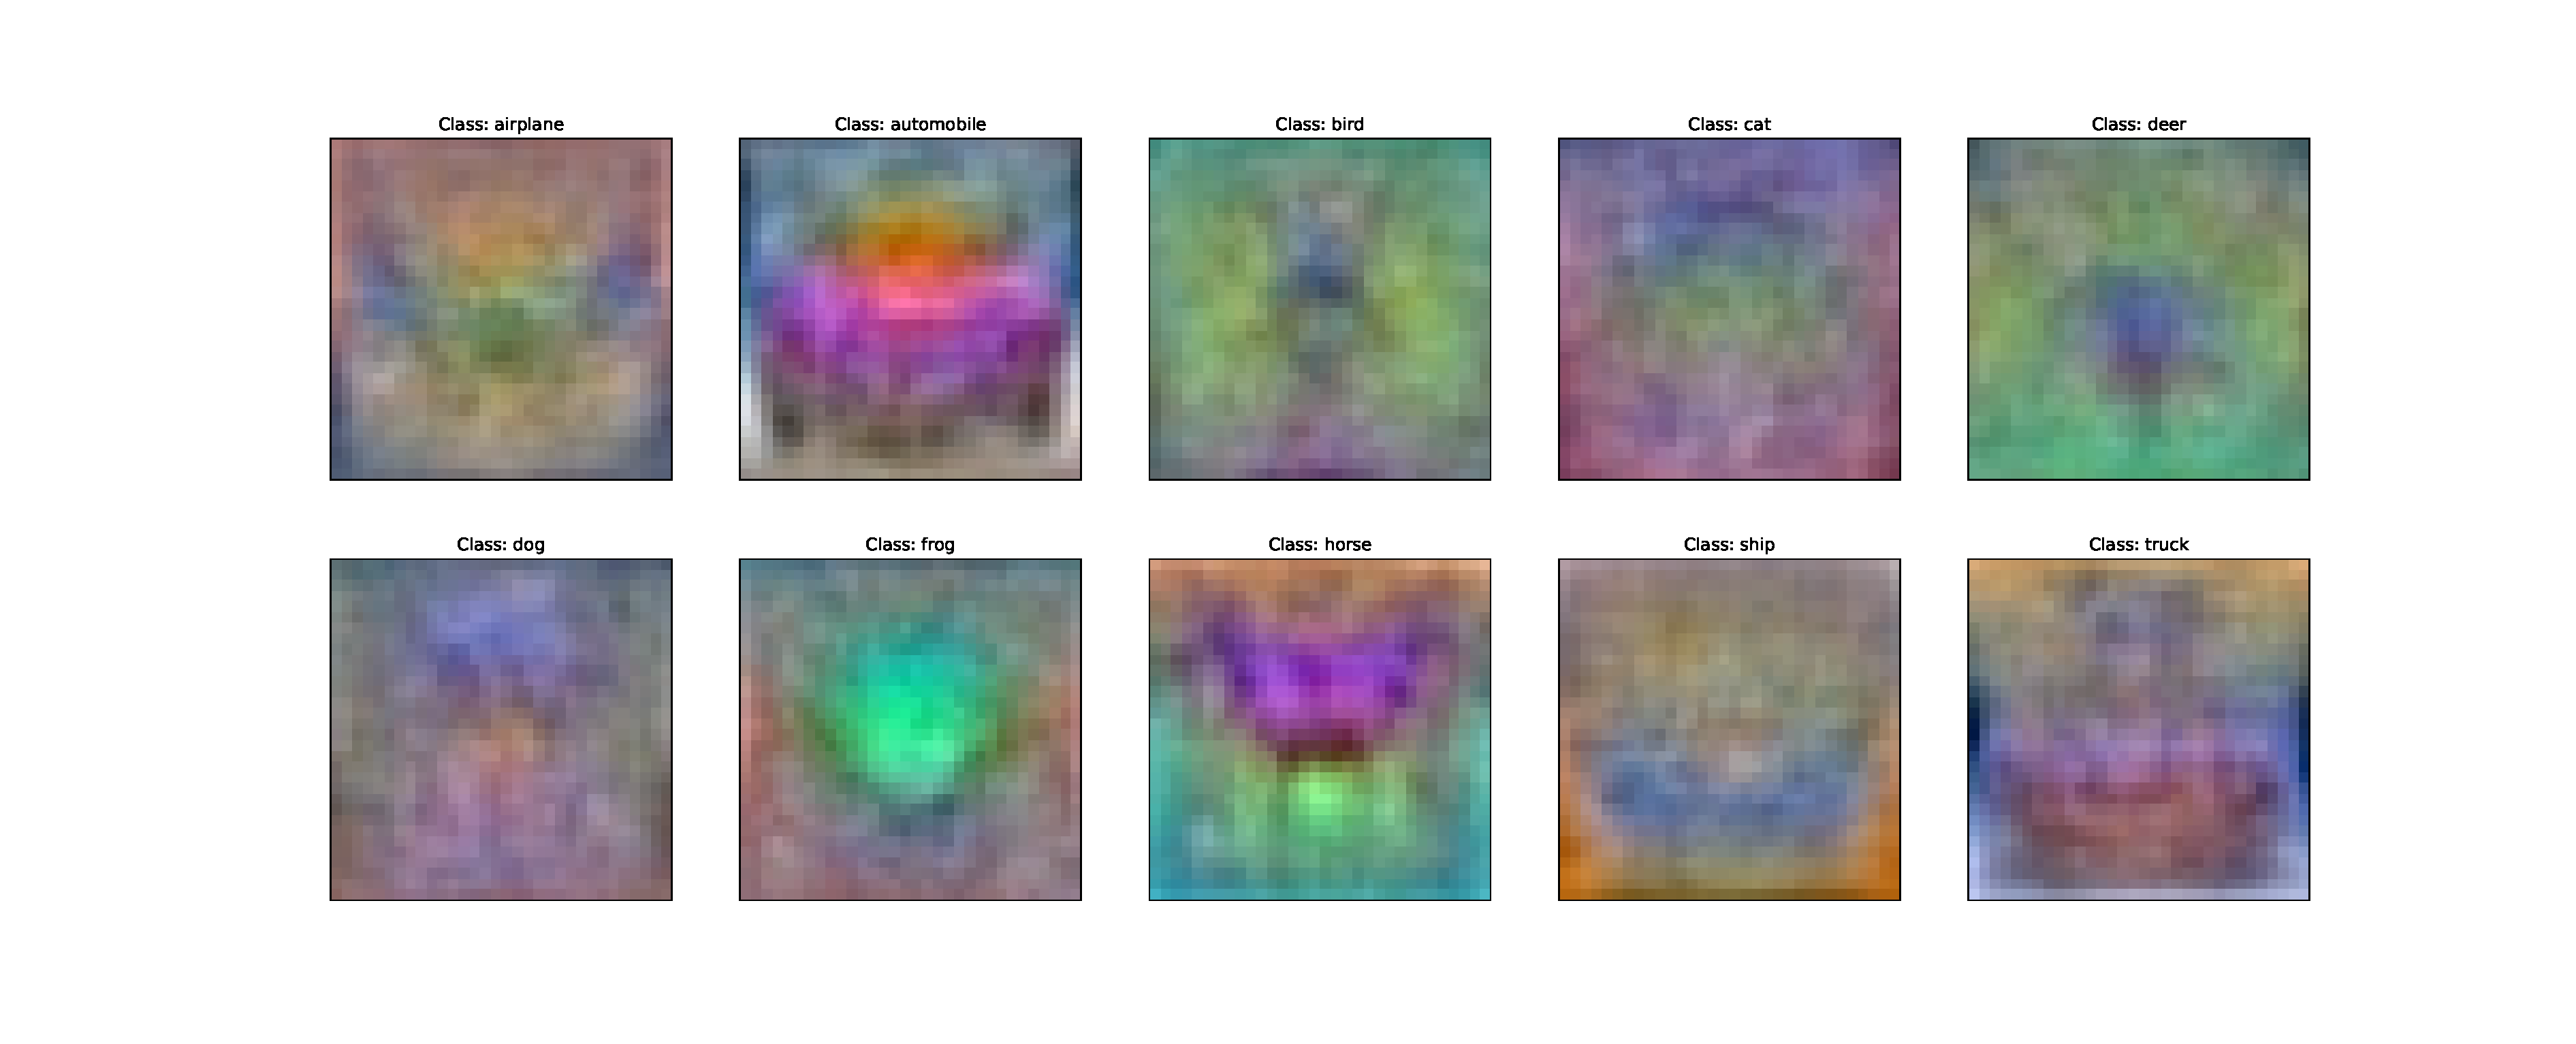
\includegraphics[scale=0.3]{figures/trainedWeightslc}
	\caption{Weights matrix W1 as 10 images}
\end{figure}

\begin{figure}[!h]
	\centering
	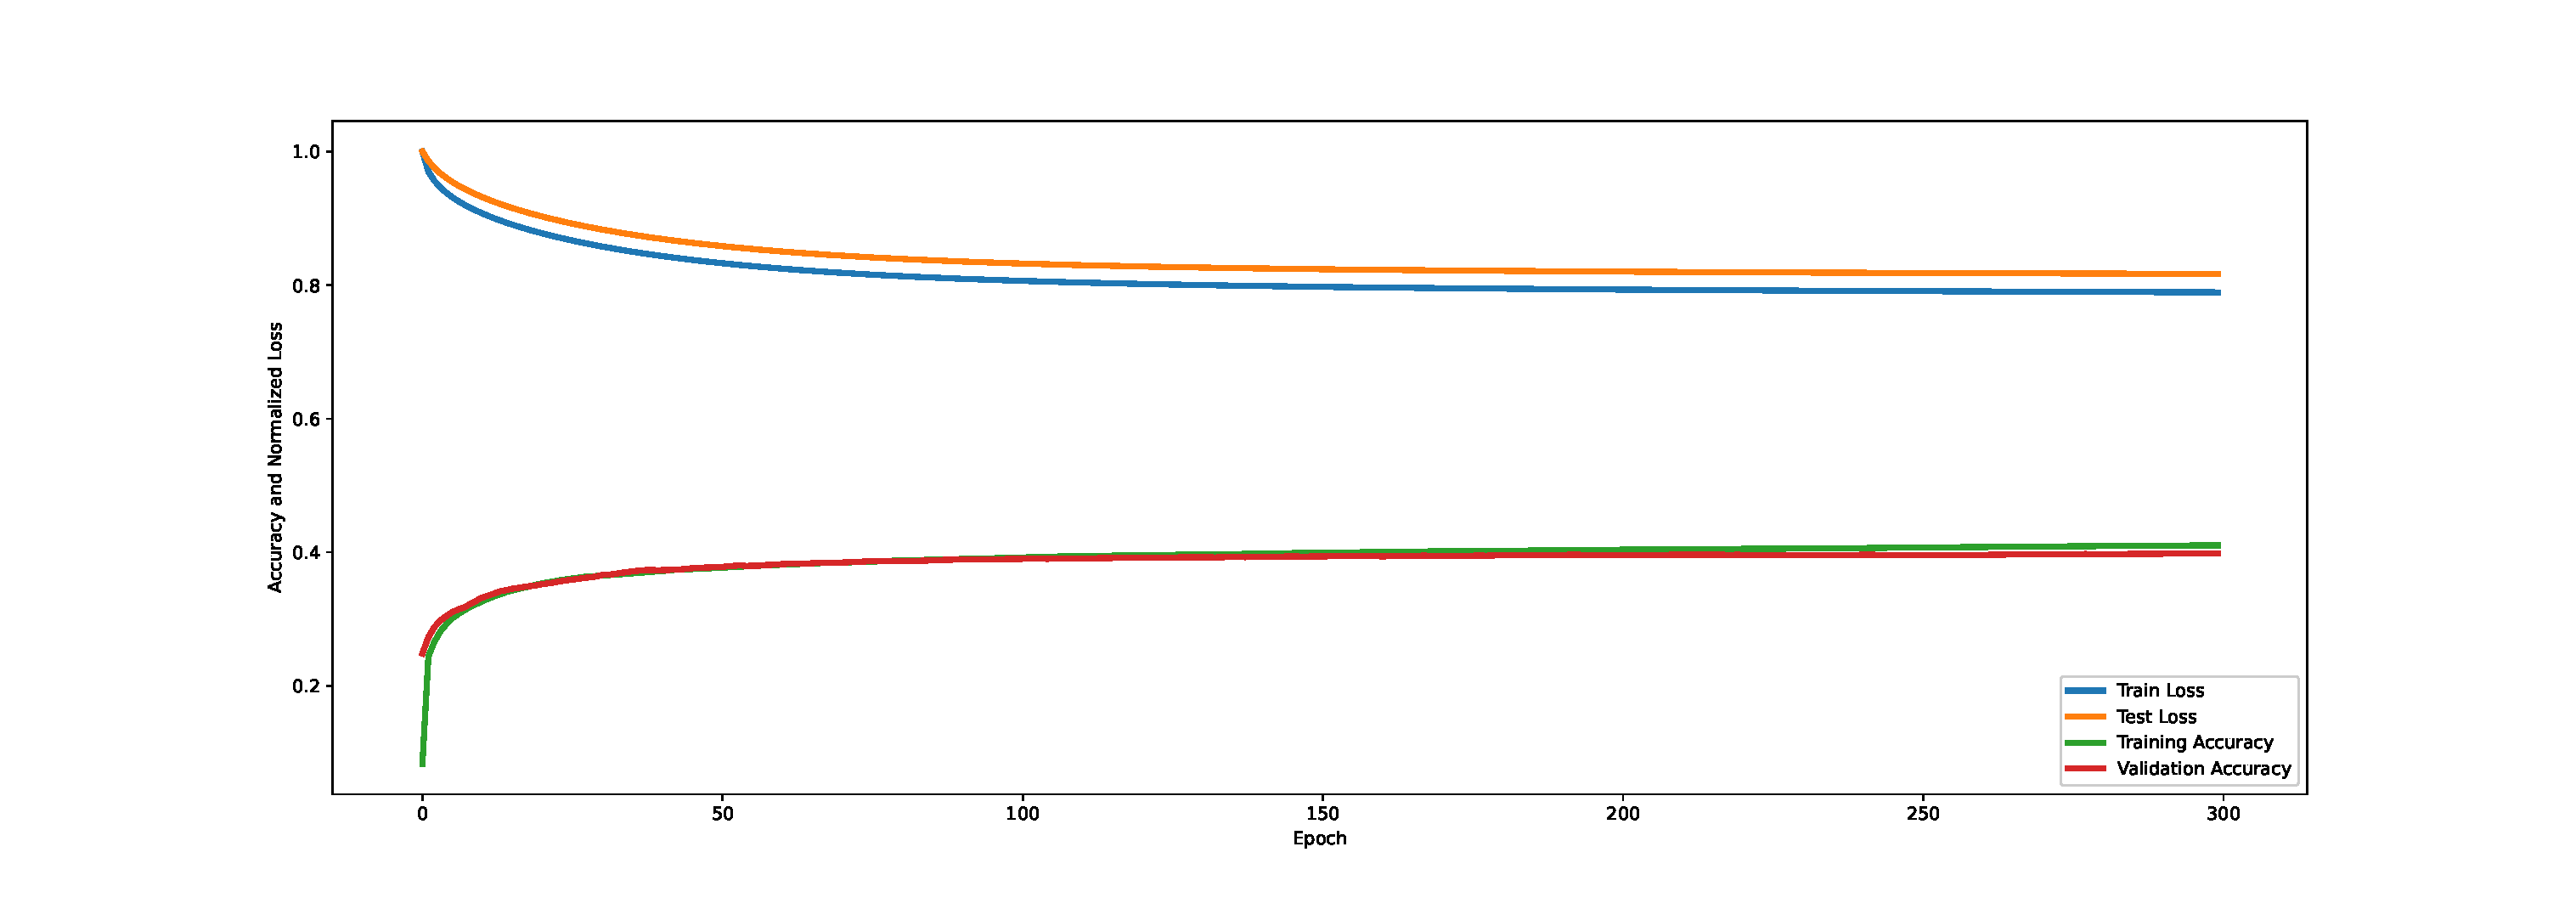
\includegraphics[scale=0.25]{figures/part1plots}
	\caption{Loss, Training Accuracy, Validation Accuracy and Learning Rate of the Linear Classifier with each iteration: for 300 epochs}
\end{figure}

\pagebreak
\section{Part 2}

\begin{figure}[!h]
	\centering
	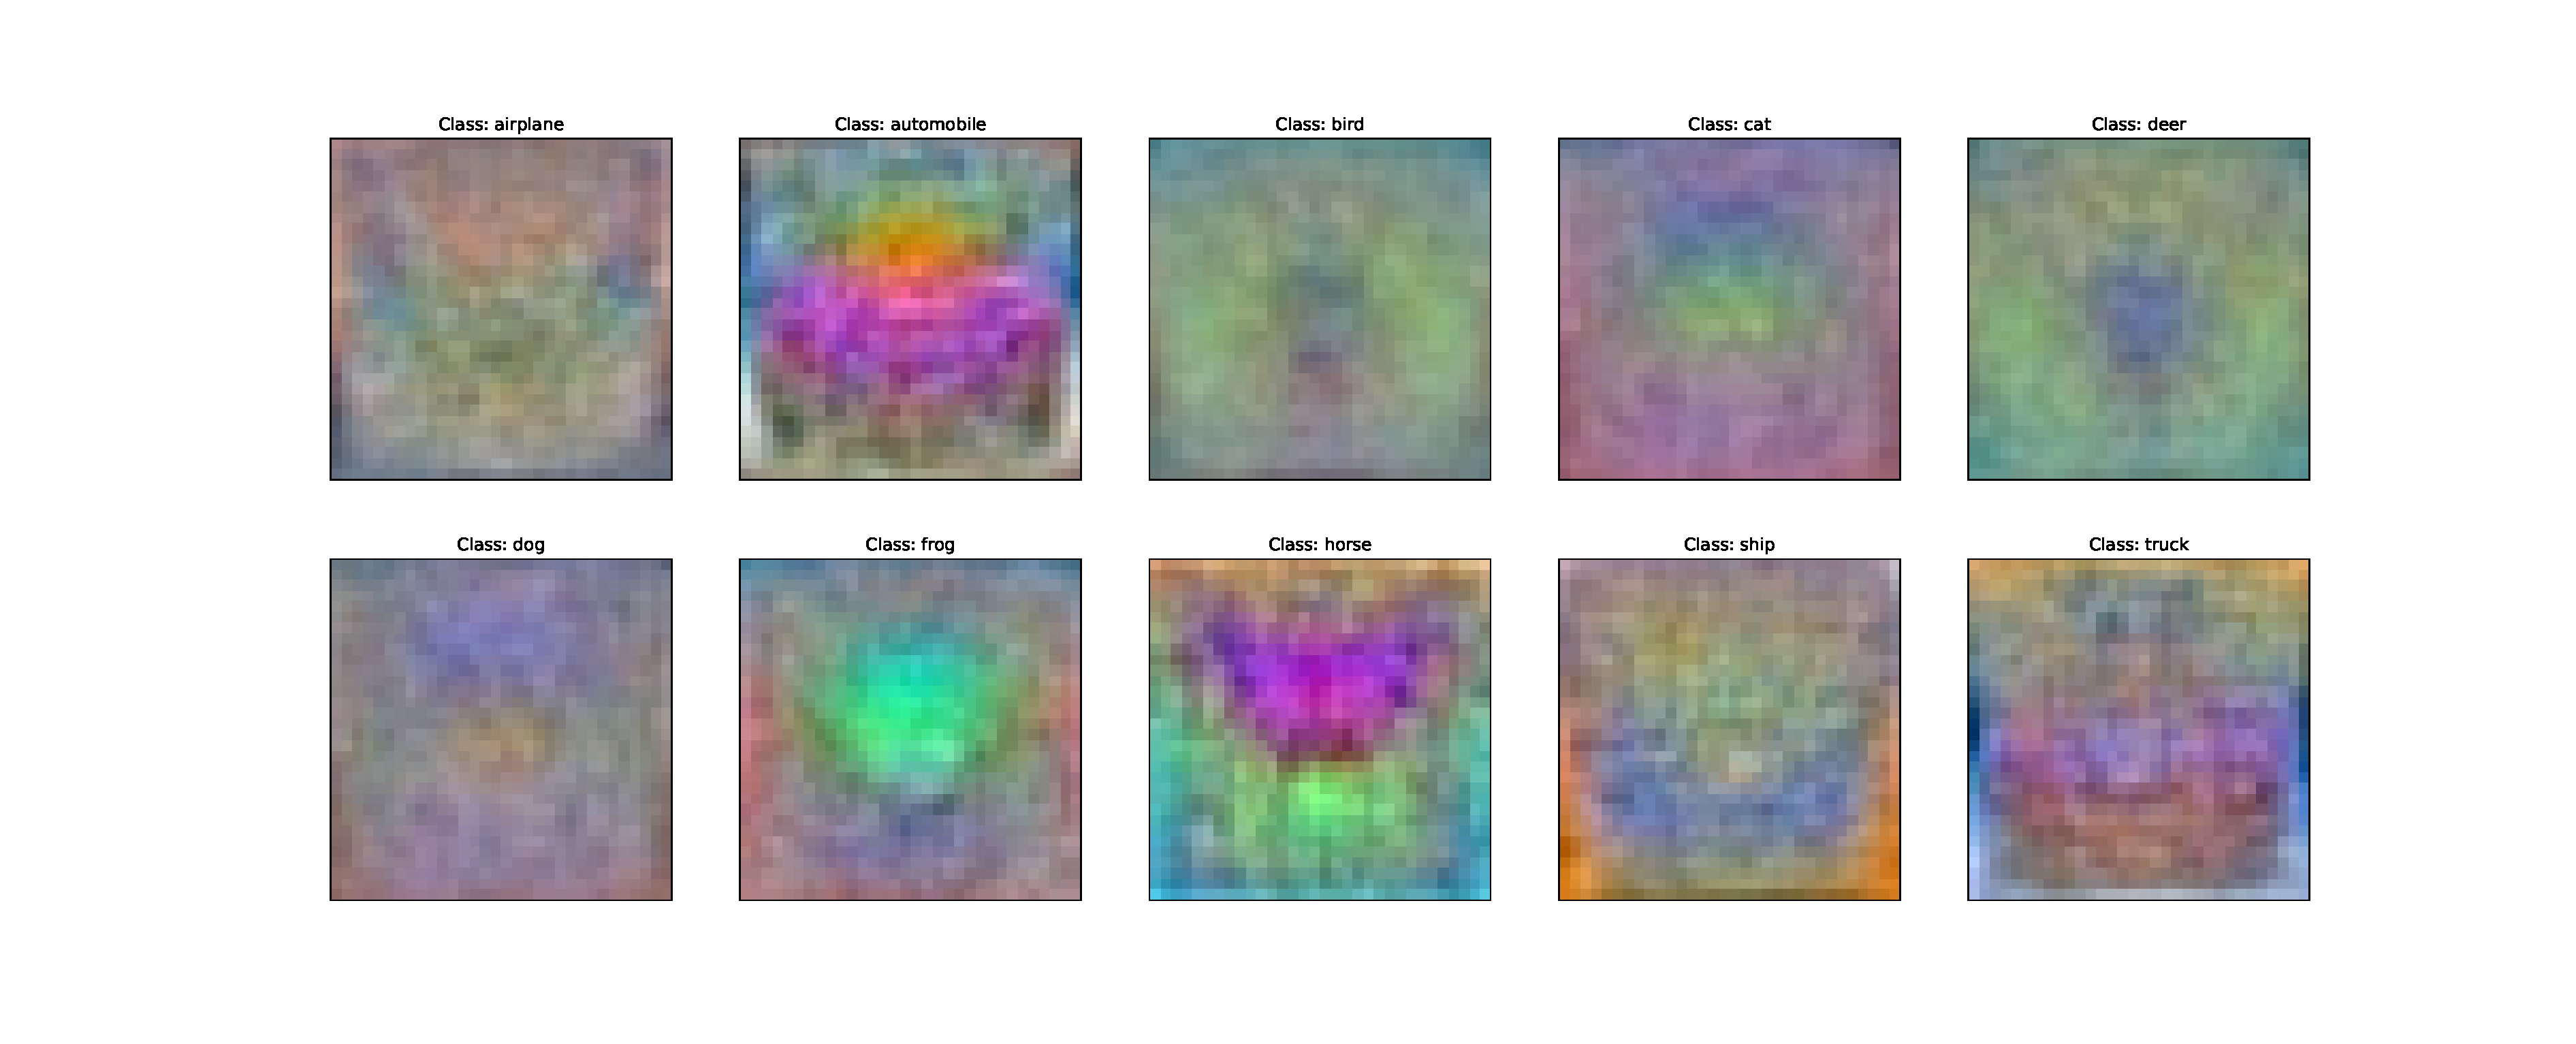
\includegraphics[scale=0.3]{figures/trainedWeightsnn2}
	\caption{Weights matrix W1 as 10 images}
\end{figure}

\begin{figure}[!h]
	\centering
	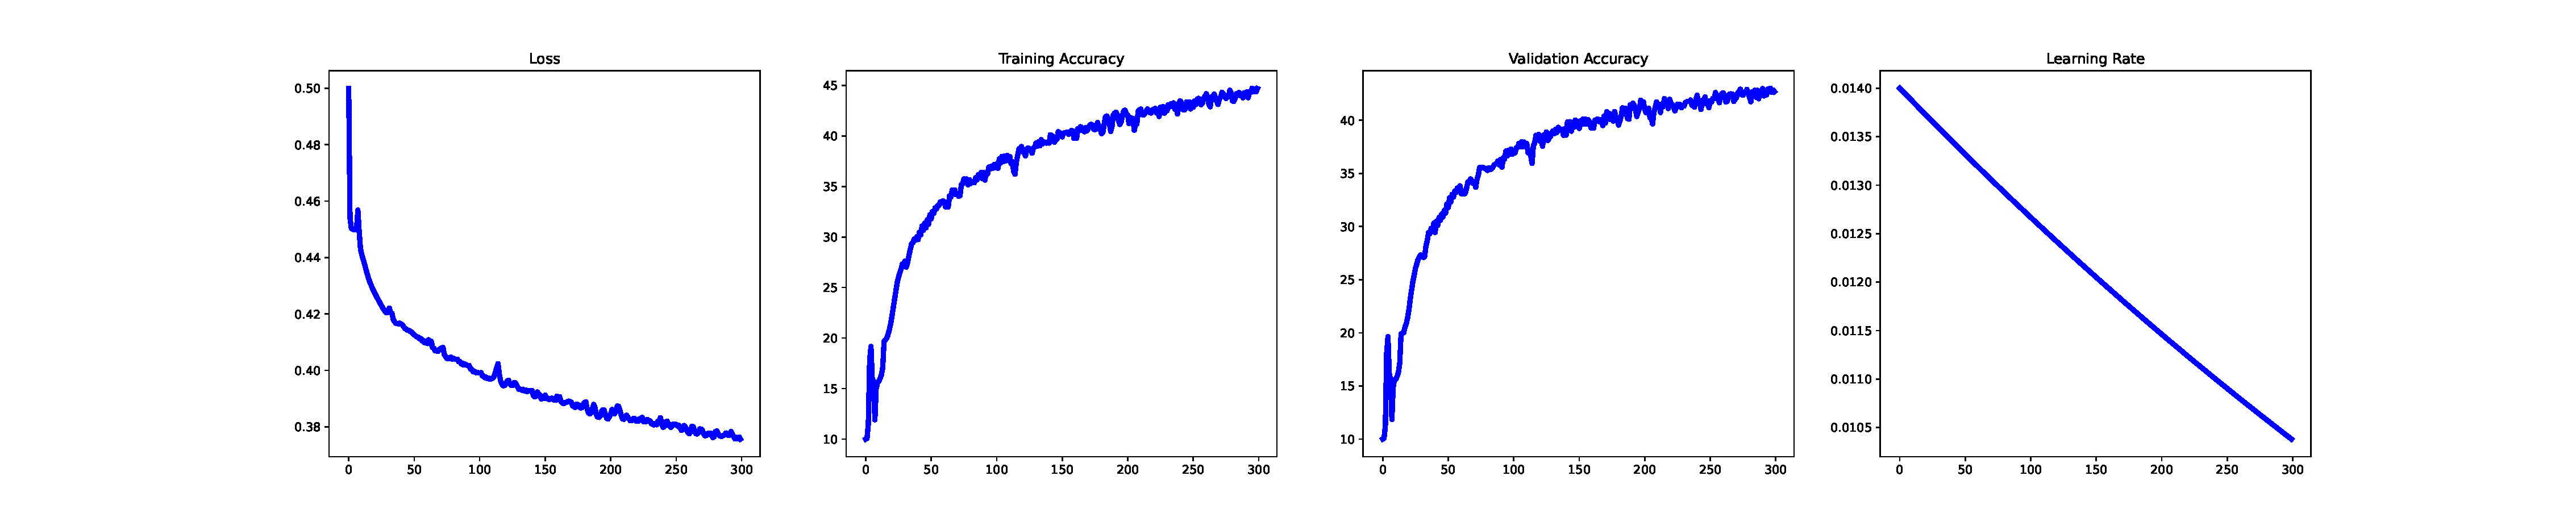
\includegraphics[scale=0.25]{figures/part2plots}
	\caption{Loss, Training Accuracy, Validation Accuracy and Learning Rate of the Linear Classifier with each iteration: for 300 epochs}
\end{figure}

\pagebreak
\section{Part 3}

\begin{figure}[!h]
	\centering
	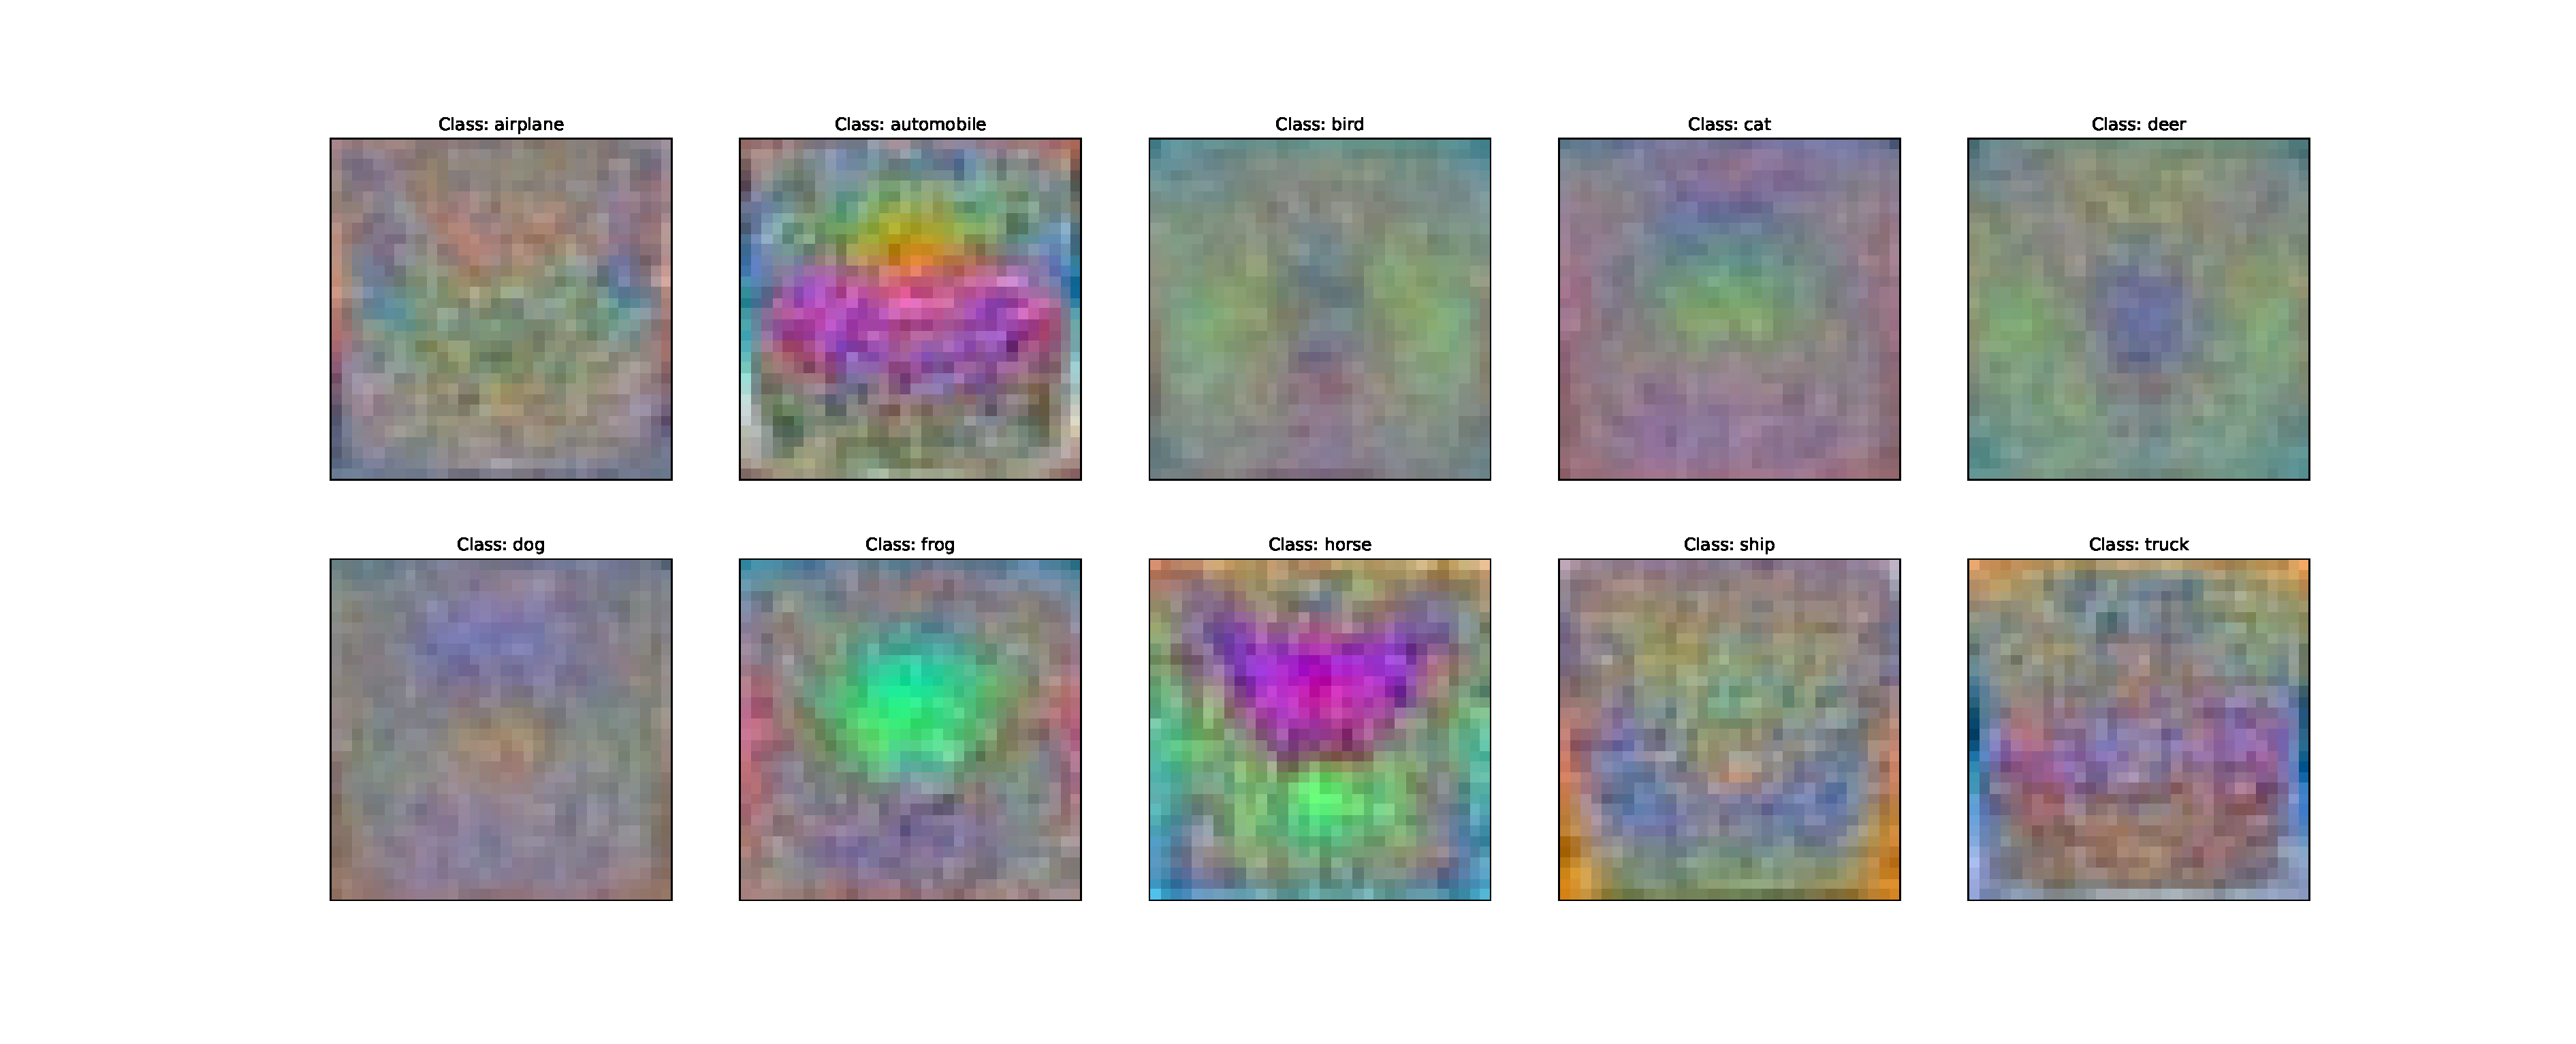
\includegraphics[scale=0.3]{figures/trainedWeightsnn2stochastic}
	\caption{Weights matrix W1 as 10 images}
\end{figure}

\begin{figure}[!h]
	\centering
	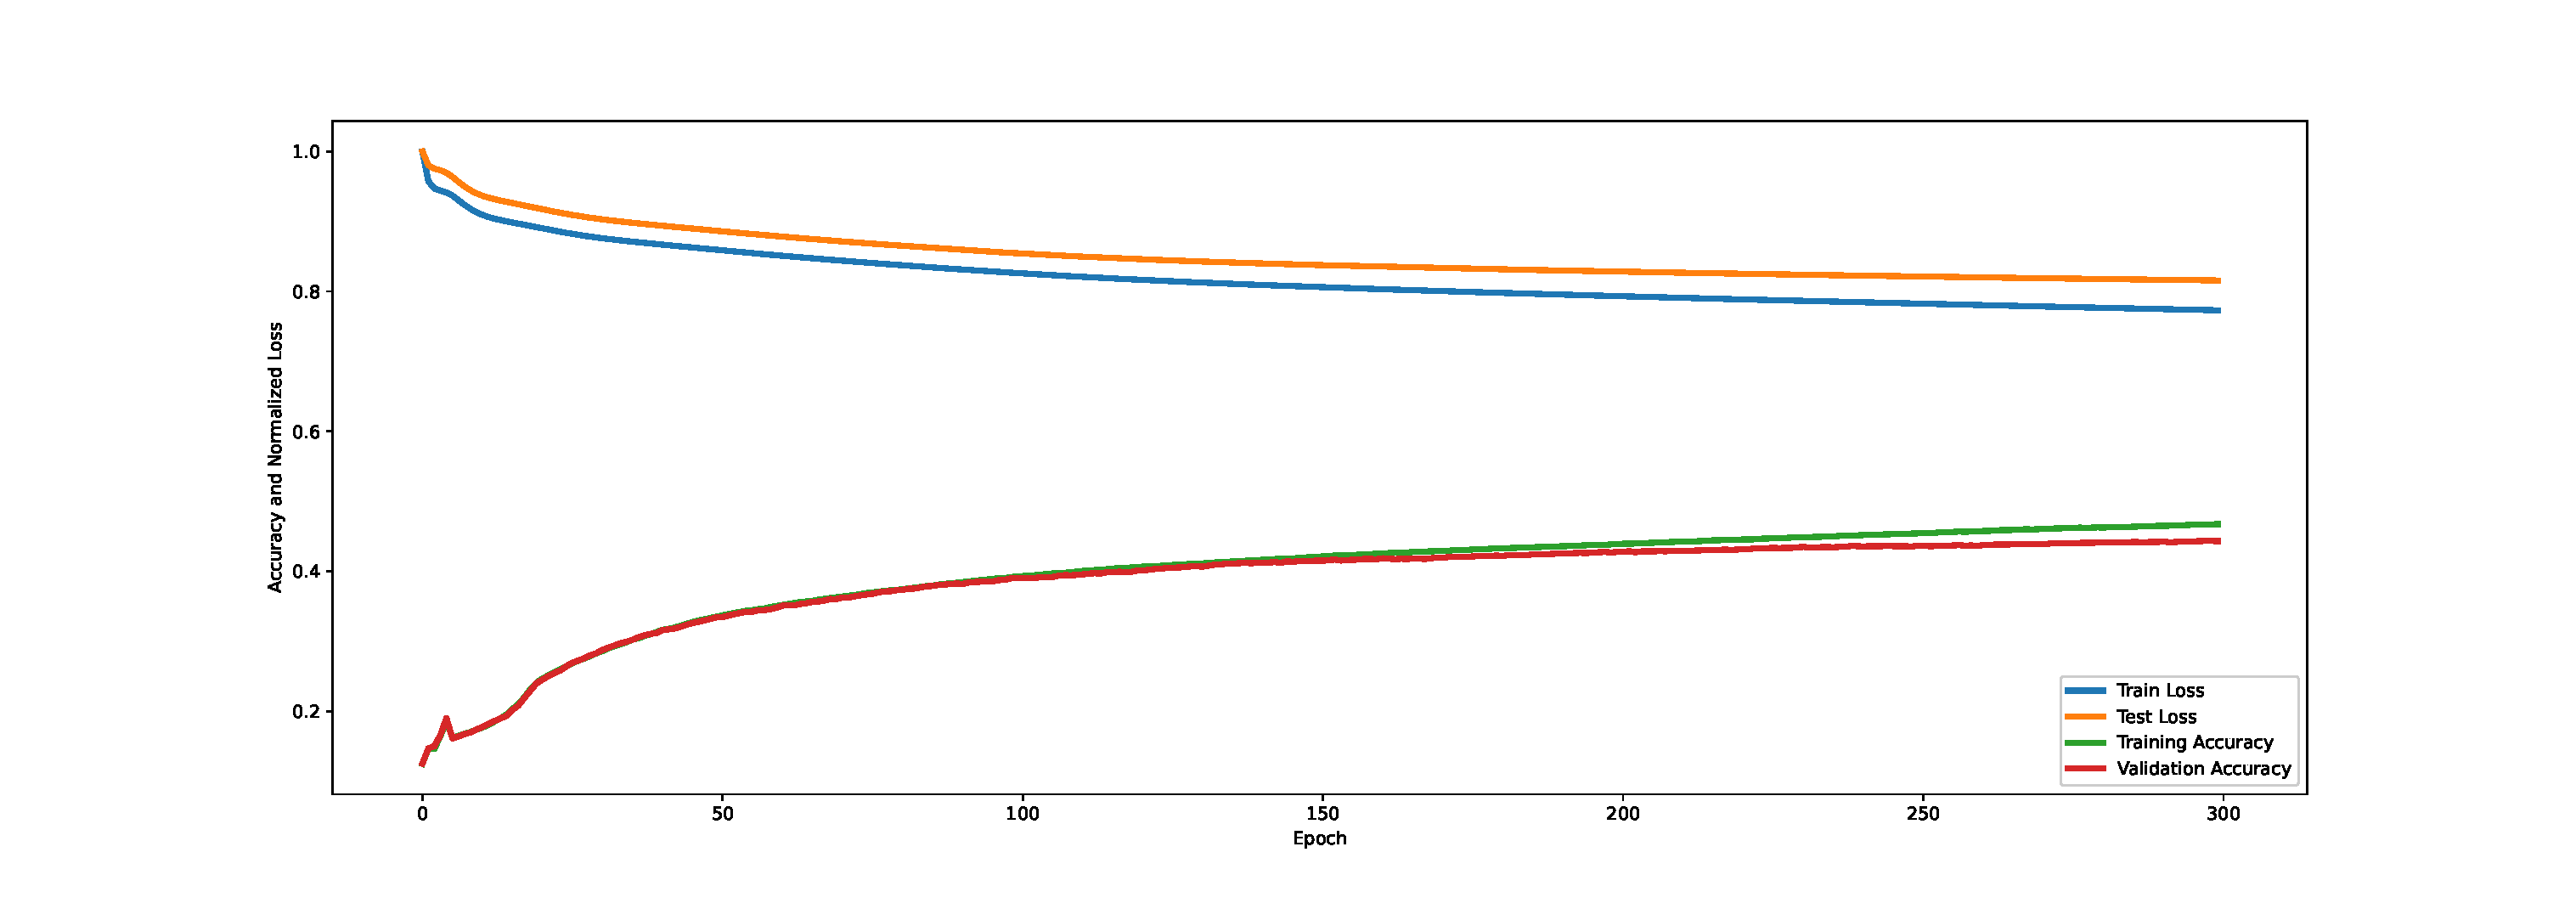
\includegraphics[scale=0.25]{figures/part3plots}
	\caption{Loss, Training Accuracy, Validation Accuracy and Learning Rate of the Linear Classifier with each iteration: for 300 epochs}
\end{figure}

\vfill
\hrule
\begin{center}
	Executable code for this assignment can be found  \href{https://github.com/bimalka98/Computer-Vision-and-Image-Processing/blob/main/EN2550Assignments/A4/180631J_a04.ipynb}{here}.
\end{center}
  
\end{document}
